\chapter{SRS - specyfikacja wymagań}

\section{Ogólny diagram przypadków użycia}

\begin{figure}[H]
	\centering
	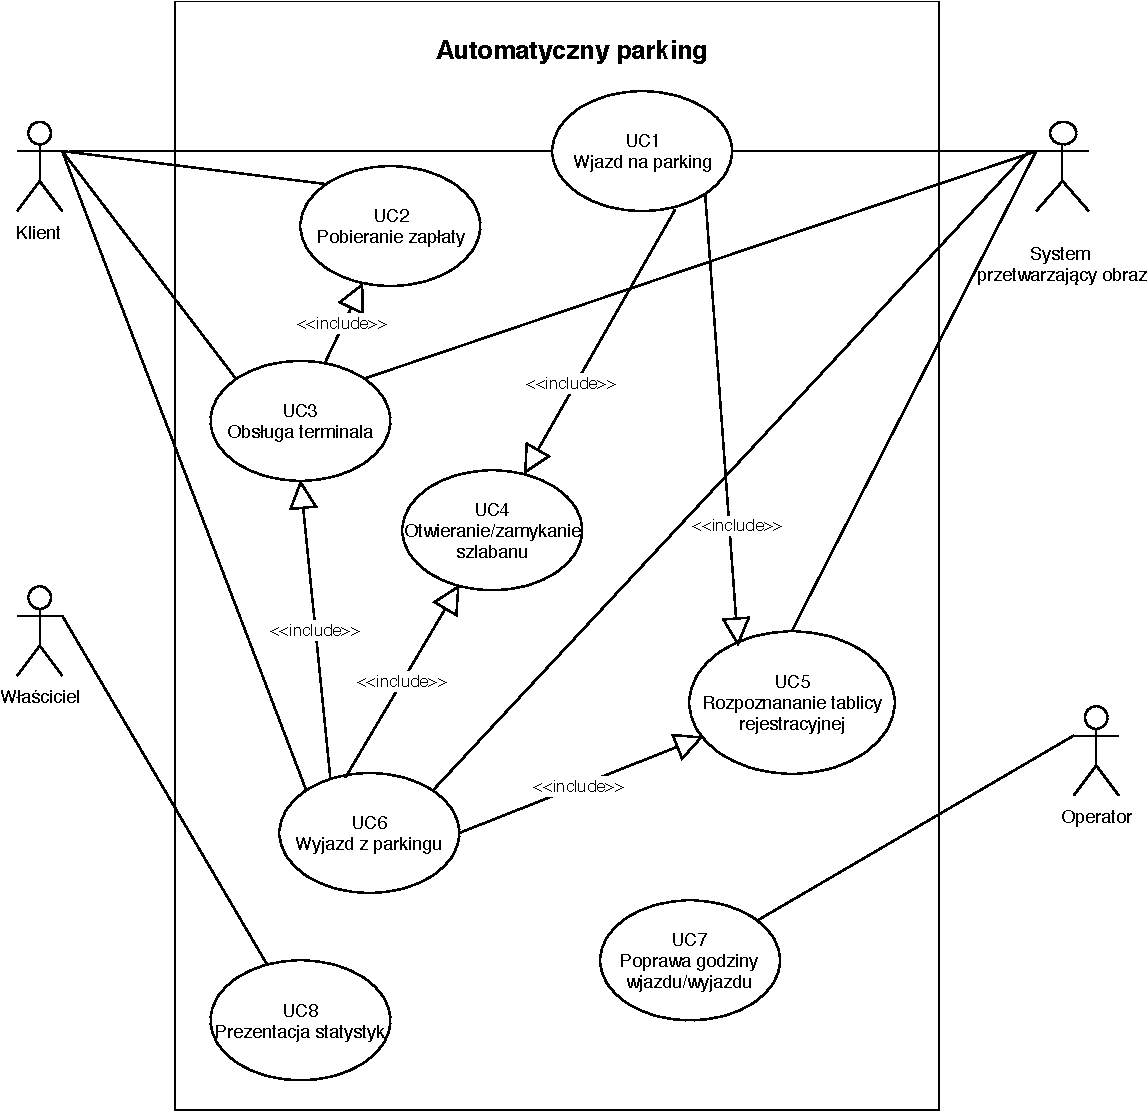
\includegraphics[width=100mm]{diagramy/PrzypUzycia.pdf}
	\caption{Przypadki użycia \label{overflow}}
\end{figure}

\section{Definicje przypadków użycia}
\subsection{Obsługa terminala (identyfikator: UC3)}
\textbf{Aktorzy: }Klient, System przetwarzający obraz

\hspace{0cm}\textbf{Zakres: }System automatycznego parkingu

\hspace{0cm}\textbf{Poziom: }Systemowy

\hspace{0cm}\textbf{Udziałowcy i ich cele: }Klient chce dokonać zapłaty za postój, system musi pobrać wszystkie niezbędne dane oraz pobrać płatność

\hspace{0cm}\textbf{Zdarzenie wyzwalające (trigger): }Klienta wybiera funkcję Zapłać za postój

\hspace{0cm}\textbf{Warunki wstępne: }Tablica rejestracyjna pojazdu klienta musi znajdować się w systemie i być poprawnie odczytana

\hspace{0cm}\textbf{Warunki końcowe dla sukcesu: }
Tablica rejestracyjna zostaje potwierdzona przez klienta, płatność zostaje potwierdzona przez system

\hspace{0cm}\textbf{Warunki końcowe dla niepowodzenia: }Tablica rejestracyjna nie zostaje potwierdzona, płatność nie zostaje przetworzona \newline

\hspace{0cm}\textbf{Scenariusz główny: }
\begin{enumerate}
\item System wyświetla formularz wprowadzania rejestracji
\item Klient wprowadza rejestrację do systemu
\item System przetwarzający obraz weryfikuje wprowadzoną rejestrację
\item System wyświetla odpowiednią rejestrację
\item Klient potwierdza zdjęcie rejestracji
\item System wyświetla kwotę do zapłaty
\item Klient dokonuje zapłaty za postój
\item System przetwarza płatność (include UC2)
\item System wyświetla potwierdzenie zapłaty
\end{enumerate}
\hspace{0cm}\textbf{Scenariusz alternatywny: }
\begin{enumerate}
\item[3.a] Wprowadzona rejestracja nie zostaje znaleziona
\item[3.a.1] Następuje powrót do punktu 1 scenariusza głównego 
\end{enumerate}
\hspace{0cm}\textbf{Scenariusz alternatywny: }
\begin{enumerate}
	\item[5.a] Klient nie potwierdza zdjęcia rejestracji
	\item[5.a.1] Następuje powrót do punktu 1 scenariusza głównego
\end{enumerate}
\hspace{0cm}\textbf{Scenariusz alternatywny: }
\begin{enumerate}
\item[8.a] Płatność nie została przetworzona poprawnie
\item[8.a.1] Następuje powrót do punktu 6 scenariusza głównego 
\end{enumerate}
\subsection{Wjazd na parking (identyfikator: UC1)}
\textbf{Aktorzy: }System przetwarzający obraz, Szlaban

\hspace{0cm}\textbf{Zakres: } System automatycznego parkingu

\hspace{0cm}\textbf{Poziom: } Systemowy

\hspace{0cm}\textbf{Udziałowcy i ich cele: } Klient chce wjechać na parking, System przetwarzający obraz musi rozpoznać tablicę rejestracyjną

\hspace{0cm}\textbf{Zdarzenie wyzwalające (trigger): } Klient podjeżdza pojazdem pod szlaban

\hspace{0cm}\textbf{Warunki wstępne: } Tablica rejestracyjna pojazdu jest widoczna i możliwa do odczytania przez system przetwarzający obraz

\hspace{0cm}\textbf{Warunki końcowe dla sukcesu: }
System przetwarzający obraz poprawnie odczytuje tablicę rejestracyjną, szlaban otwiera się

\hspace{0cm}\textbf{Warunki końcowe dla niepowodzenia: } System przetwarzający obraz nie może odczytać tablicy rejestracyjnej, szlaban nie otwiera się \newline

\hspace{0cm}\textbf{Scenariusz główny: }
\begin{enumerate}
\item System przetwarzający obraz robi zdjęcie
\item System przetwarzający obraz odczytuje tablicę rejestracyjną
\item System automatycznego parkingu zapisuje datę i czas wjazdu pojazdu
\item Szlaban otwiera się (include: UC4)
\item Klient wjeżdża na parking
\item Szlaban zamyka się (include: UC4)
\end{enumerate}
\hspace{0cm}\textbf{Scenariusz alternatywny: }
\begin{enumerate}
\item[2.a] System przetwarzający obraz nie może odczytać tablicy rejestracyjnej
\item[2.a.1] Następuje powrót do punktu 1 scenariusza głównego
\end{enumerate}


\subsection{Wyjazd z parkingu (identyfikator: UC5)}
\textbf{Aktorzy: }System przetwarzający obraz, Szlaban

\hspace{0cm}\textbf{Zakres: }System automatycznego parkingu

\hspace{0cm}\textbf{Poziom: }Systemowy

\hspace{0cm}\textbf{Udziałowcy i ich cele: }Klient chce wyjechać z parkingu

\hspace{0cm}\textbf{Zdarzenie wyzwalające (trigger): } System odlicza 15 minut na wyjazd z parkingu

\hspace{0cm}\textbf{Warunki wstępne: }
Rejestracja pojazdu została poprawnie odczytana przy wjeździe

\hspace{0cm}\textbf{Warunki końcowe dla sukcesu: }Klient opuścił parking

\hspace{0cm}\textbf{Warunki końcowe dla niepowodzenia: }Klient nie opuścił parkingu \newline

\hspace{0cm}\textbf{Scenariusz główny: }
\begin{enumerate}
\item Klient obsługuje terminal (inlcude: UC3)
\item System potwierdza możliwość wyjazdu w ciągu 15 minut
\item System przetwarzający obraz ponownie robi zdjęcie
\item System przetwarzający obraz rozpoznaje tablicę rejestracyjną
\item System automatycznego parkingu weryfikuje dane: numer rejestracyjny, potwierdzenie płatności, pozostały czas wyjazdu
\item Szlaban otwiera się (include: UC4)
\item Klient opuszcza parking
\item Szlaban zamyka się (include: UC4)
\end{enumerate}
\hspace{0cm}\textbf{Scenariusz alternatywny: }
\begin{enumerate}
\item[4.a] System przetwarzający obraz nie może rozpoznać tablicy rejestracyjnej
\item[4.a.1] Następuje powrót do punktu 3 scenariusza głównego
\end{enumerate}

\hspace{0cm}\textbf{Scenariusz alternatywny: }
\begin{enumerate}
\item[5.a] Płatność nie została potwierdzona
\item[5.a.1] Następuje powrót do punktu 1 scenariusza głównego
\end{enumerate}

\hspace{0cm}\textbf{Scenariusz alternatywny: }
\begin{enumerate}
\item[5.a] Czas na wyjazd z parkingu skończył się
\item[5.a.1] Następuje powrót do punktu 1 scenariusza głównego
\end{enumerate}

\subsection{Prezentacja statystyk (identyfikator: UC8)}
\textbf{Aktorzy: }Właściciel

\hspace{0cm}\textbf{Zakres: }System automatycznego parkingu

\hspace{0cm}\textbf{Poziom: }systemowy

\hspace{0cm}\textbf{Udziałowcy i ich cele: } Właściciel chce wyświetlić statystyki

\hspace{0cm}\textbf{Zdarzenie wyzwalające (trigger): } Właściciel wywołuje funkcję Pokaż statystyki

\hspace{0cm}\textbf{Warunki wstępne: }
Właściciel musi być zalogowany

\hspace{0cm}\textbf{Warunki końcowe dla sukcesu: } System prezentuje wybrane statystyki

\hspace{0cm}\textbf{Warunki końcowe dla niepowodzenia: } System nie może wyświetlić wybranych statystyk, błędne dane \newline

\hspace{0cm}\textbf{Scenariusz główny: }
\begin{enumerate}
\item System wyświetla rodzaje statystyk do wyboru: dzienne, miesięczne, roczne
\item Właściciel wybiera odpowiedni rodzaj statystyk
\item System oblicza wybrane statystyki
\item System prezentuje wyniki
\end{enumerate}
\hspace{0cm}\textbf{Scenariusz alternatywny: }
\begin{enumerate}
\item[3.a] System nie może wyświetlić wybranych statystyk
\item[3.a.1] Właściciel poprawia błędne dane w systemie
\item[3.a.2] Następuje powrót do punktu 1 scenariusza głównego
\end{enumerate}

\subsection{Poprawa danych w systemie (identyfikator: UC7)}
\textbf{Aktorzy: }Operator

\hspace{0cm}\textbf{Zakres: }System automatycznego parkingu

\hspace{0cm}\textbf{Poziom: }Systemowy

\hspace{0cm}\textbf{Udziałowcy i ich cele: }Operator chce poprawić błędne dane w systemie

\hspace{0cm}\textbf{Zdarzenie wyzwalające (trigger): }Operator wywołuje funkcję Popraw dane

\hspace{0cm}\textbf{Warunki wstępne: }
Operator musi byc zalogowany

\hspace{0cm}\textbf{Warunki końcowe dla sukcesu: }Do systemu zostają wprowadzone poprawne dane

\hspace{0cm}\textbf{Warunki końcowe dla niepowodzenia: }System nie może przetworzyć nowych danych\newline

\hspace{0cm}\textbf{Scenariusz główny: }
\begin{enumerate}
\item System wyświetla formularz poprawiania danych
\item Operator wprowadza poprawione dane: numer rejestracyjny, godzinę wjazdu/wyjazdu, datę wjazdu/wyjazdu
\item System przetwarza wprowadzone dane
\item System wyświetla potwierdzenie zmian
\end{enumerate}

\hspace{0cm}\textbf{Scenariusz alternatywny: }
\begin{enumerate}
\item[3.a] system nie może przetworzyć nowych danych
\item[3.a.1] System wyświetla ponownie formularz, znaznaczając które pola zostały niepoprawnie wypełnione
\item[3.a.2] Następuje powrót do punktu 3 scenariusza głównego
\end{enumerate}